\documentclass[12pt, a4paper]{article}
\usepackage{ctex}  % 支持中文
\usepackage{amsmath, amssymb}  % 数学符号和公式
\usepackage{graphicx}  % 插入图片
\usepackage{geometry}  % 页面设置
\usepackage{booktabs}  % 表格美化
\usepackage{tabularx}  % 表格宽度自适应
\usepackage{multirow}  % 合并单元格
\usepackage{enumitem}  % 列表设置
\usepackage{caption}   % 标题设置
\usepackage{array}     % 表格增强
\usepackage{fancyhdr}  % 页眉页脚
\usepackage{titlesec}  % 标题格式设置
\usepackage{fontspec}

\usepackage[
  backend=bibtex,
  style=gb7714-2015,   % 使用中国国标格式,适合中文论文
  sorting=none         % 按引用顺序排序
]{biblatex}

\addbibresource{references.bib} % 参考文献配置

% 页面设置
\geometry{left=2.5cm, right=2.5cm, top=2.5cm, bottom=2.5cm}

% 重定义section格式为居中
\titleformat{\section}{\centering\Large\bfseries}{\thesection}{1em}{}
\titleformat{\subsection}{\normalsize\bfseries}{\thesubsection}{1em}{}
\titleformat{\subsubsection}{\normalsize\bfseries}{\thesubsubsection}{1em}{}

% 表格表头格式
\renewcommand{\thetable}{\arabic{section}.\arabic{table}}

% 设置表格标题格式:左对齐,中文带"表"字,表题加粗
\captionsetup[table]{
  labelsep=space,
  labelformat=simple,
  textfont=bf,
  labelfont=bf,
  name=表
}

% 图片编号格式
\renewcommand{\thefigure}{\arabic{section}-\arabic{figure}}

% 设置图片标题格式
\captionsetup[figure]{
  labelsep=space,
  labelformat=simple,
  textfont=bf,     
  labelfont=bf, 
  position=bottom,  
  name=图
}

% 修改公式编号格式
\renewcommand{\theequation}{\thesection-\arabic{equation}}

% 参考文献格式
\makeatletter
\renewcommand\@biblabel[1]{[#1]}
\makeatother

\begin{document}

% 标题部分
\begin{center}
\LARGE\textbf{中国股市收益率的分布特征}

\vspace{1cm}
\large 计金220 22011854 高菻铠
\end{center}

\noindent \textbf{摘要:} 本文基于上证指数分钟级高频数据,对中国股市收益率分布特征展开多尺度实证研究。研究采用1至240分钟七个时间尺度的收益率序列,通过概率密度估计、正态性检验及尾部特征分析等方法,系统探究了收益率分布特性的动态演化规律。研究发现,中国股市收益率分布呈现显著的尖峰胖尾特征,且尾部符合“负三次方定律”。KS检验表明,所有时间尺度下分布均显著偏离正态性,偏离程度随尺度扩大呈指数衰减。Hurst指数($H$=0.27)显示市场存在均值回归特性,支持过度反应假说。研究进一步显示,极端事件发生机制具有尺度依赖性:1分钟、60分钟和120分钟尺度符合幂律分布,而中间时间尺度(5-30分钟)的尾部指数异常升高。这些发现为新兴市场的风险管理提供了跨尺度的理论框架。研究发现为风险管理和投资决策提供了实证依据,具有重要理论与现实意义。

\section{文献综述}

金融市场收益率分布特征的研究一直是金融物理学和量化金融的核心议题。传统金融理论假设资产收益率服从正态分布,但大量实证研究表明,金融市场收益率分布通常表现出显著的非正态特征,如"尖峰胖尾"分布和幂律特性\cite{du2007}。这些特征体现了金融市场作为复杂系统的非线性动力学特性,对风险管理和金融衍生品定价具有重要影响。

\citet{ghashghaie1996}在《Nature》期刊上发表的研究首次揭示了外汇市场收益率波动与湍流理论之间的相似性,发现金融市场信息级联传递过程与湍流中能量级联传递机制具有相似的动力学特征。该研究通过对比分析不同时间尺度下的外汇收益率差异,证实了收益率分布的尺度不变性并发现概率密度服从某种幂律关系。

在中国股票市场研究方面,\citet{du2007}对上证综指和深证成指在六种时间尺度(1分钟至60分钟)的高频数据进行实证分析,发现收益率分布具有明显的尖峰胖尾特征。研究表明上证综指每分钟收益率的概率分布和累积概率分布均符合幂律关系,特征指数分别为2.86和2.31,超出了Lévy稳定分布的范围。该研究还发现Lévy稳定分布能较好地描述收益率概率分布的中间区域,上证综指和深证成指的Lévy指数分别为1.26和1.74,均属于非线性分形系统。

\citet{chen2008}进一步扩展了这项研究,以上海证券交易所综合指数(SSECC)为研究对象,通过5分钟和1天两个时间尺度的数据分析,研究收益率的多标度幂律特征和临界现象。研究发现收益率分布的中心部分符合Lévy分布,Lévy指数在$0<\alpha<2$范围内;而分布尾部符合另一种幂律关系,特征指数$\alpha\approx3$。这表明中国股市具有与成熟市场相似的统计特性。该研究还发现在时间尺度$\Delta t>4\text{days}$时,收益率分布逐渐趋近于正态分布,展现出与成熟市场$\Delta t\approx4\text{days}$临界值相一致的特性。

综合这些研究可以看出,金融市场作为复杂的非线性系统,其收益率分布普遍表现出尖峰胖尾和幂律特性。中国股票市场虽然相对年轻,但收益率分布特征与国际成熟市场具有显著相似性,体现了某种金融市场的普适规律。特别是Lévy指数和幂律指数的定量分析结果表明,中国股市可能具有更强的波动性和极端风险,这对投资决策和风险管理具有重要指导意义。

在不同时间尺度下,收益率分布展现出明显的标度不变性和多分形特征。随着时间尺度增加,收益率分布逐渐向正态分布靠近,表明金融市场存在某种自组织临界状态。研究还发现,Hurst指数小于0.5,表明收益率序列存在反持续性和均值回归趋势,这表明市场具有过度反应和修正的特性\cite{du2007}。

上述文献综述显示了金融市场收益率分布的非正态特性及其多尺度演化规律。基于此,本研究采用上证指数高频数据,通过多尺度分析方法进一步探究中国股市收益率的分布特征。具体而言,我们聚焦于1至240分钟时间尺度下的动态演化规律,结合涨跌停制度特征,系统分析尖峰胖尾特性、尾部幂律行为及标度不变性。研究旨在为中国股市的风险管理和投资决策提供更精细化的实证依据。

\section{数据与方法}

\subsection{数据描述}

本研究采用上证指数(Shanghai Stock Exchange Composite Index, SSEC)的分钟级价格数据进行实证分析。原始数据集经初步筛选后包含共计715,138个有效数据点,数值范围在998.337至6122.674之间,具有较高的市场代表性和时间分辨率。我们通过标记过滤方法剔除了价格为0的异常数据点,保证价格序列的有效性。数据预处理过程采用Python语言实现,通过NumPy和Pandas库进行矩阵运算与数据框操作,加速了大规模高频数据的处理效率。

\subsection{收益率计算与多尺度划分}

基于金融市场微观结构理论,我们构建了一个完整的多尺度分析框架,选取七个典型的时间尺度$\Delta t$(分别为1, 5, 10, 30, 60, 120和240分钟),计算对数收益率:

\begin{equation}
r_{\Delta t}(t) = \ln P(t+\Delta t) - \ln P(t)
\end{equation}

其中$P(t)$表示时间$t$的价格。对数收益率的选择基于其良好的统计特性,包括时间可加性和对数正态价格假设下的理论意义。同时,对数收益率的计算过程在Python环境中通过NumPy的向量化操作实现,大幅优化了计算效率:

\begin{verbatim}
r = np.log(mat_data[scale:]) - np.log(mat_data[:-scale])
\end{verbatim}

为稳健分析并考虑中国股市的制度特征,我们对收益率进行了过滤,仅保留-0.1到0.1之间的值,对应于中国股市的涨跌停限制机制。过滤过程通过条件筛选实现:

\begin{verbatim}
r_filter = []
for value in r:
    if value >= -0.1 and value <= 0.1:
        r_filter.append(value)
r_filter = np.array(r_filter)
\end{verbatim}

上述的多尺度划分方法能够全面捕捉市场在不同时间尺度上的动态特性,从高频交易噪声到中长期趋势,为研究收益率分布特征随时间尺度演化提供了完整框架。

\subsection{经验概率密度估计的非参数方法}

本研究采用非参数化方法精确估计各时间尺度收益率的经验概率密度函数。根据统计理论,我们将收益率样本覆盖的范围分成均匀区间$[r_{i-1}, r_i]$,计算每个区间内的样本个数$y_i$,并根据如下公式估计概率密度:

\begin{equation}
p_i = \frac{y_i}{(r_i-r_{i-1}) \cdot m}
\end{equation}

其中$m$为样本总数,$(r_i-r_{i-1})$为区间宽度,确保了概率密度函数的积分为1。概率密度计算过程在Python中通过以下自定义函数实现:

\begin{verbatim}
def calc_empirical_probability(data, num_bin):
    """
    计算数据的经验概率密度函数
    参数:
    data - 收益率数据
    num_bin - 区间划分数量
    
    实现逻辑:
    1. 将数据范围等分为num_bin个区间
    2. 计算每个区间中点作为横坐标
    3. 统计各区间样本数并计算概率密度
    4. 过滤零概率密度点以保证数值稳定性
    """
    bin = np.linspace(np.min(data), np.max(data), num_bin)
    x_emp = np.zeros(len(bin) - 1)
    y_emp = np.zeros(len(bin) - 1)
    
    for i in range(len(bin) - 1):
        x_emp[i] = (bin[i] + bin[i+1]) / 2
        y_emp[i] = np.sum((data >= bin[i]) & (data < bin[i+1])) / len(data) / (bin[i+1] - bin[i])
    
    # 只保留概率密度大于0的点
    mark = y_emp > 0
    x_emp = x_emp[mark]
    y_emp = y_emp[mark]
    
    return x_emp, y_emp
\end{verbatim}

在实际估计过程中,我们采用了301个划分点形成300个分析区间,这能够在保证分辨率的同时有效抑制随机波动对估计精度的干扰。为突出分布尾部特征,我们采用半对数坐标系进行可视化处理,使用Matplotlib库的semilogy函数实现,纵轴跨度设定为$[10^{-4}, 10^3]$,能够对极端事件概率的精确刻画,同时通过标记点和连线的组合增强了视觉效果。

\subsection{正态拟合与分布偏离度检验方法}

为量化不同时间尺度收益率分布与正态分布的偏离程度,我们结合参数估计和假设检验方法进行系统分析。首先,使用SciPy库中的norm.fit函数对各时间尺度的收益率序列进行最大似然估计,获得均值$\mu$和标准差$\sigma$参数:

\begin{verbatim}
mu, sigma = norm.fit(returns)
\end{verbatim}

随后,我们构建相应的正态概率密度函数:

\begin{verbatim}
x_fit = np.linspace(-0.1, 0.1, 300)
y_fit = norm.pdf(x_fit, loc=mu, scale=sigma)
\end{verbatim}

为客观评价拟合程度,我们采用Kolmogorov-Smirnov (KS)检验,这是一种非参数检验方法,通过比较实证分布与理论分布的最大偏离度来评估拟合优度:

\begin{verbatim}
ks_statistic, p_value = kstest(returns, 'norm', args=(mu, sigma))
\end{verbatim}

KS检验不依赖于数据分布假设,对样本量大小不敏感,能够提供更为稳健的检验结果。我们系统分析了KS统计量随时间尺度的变化趋势,以揭示收益率分布向正态分布靠近的规律与特性。

\subsection{幂律分布拟合与尾部特征分析}

针对收益率分布的尾部特征,我们采用复杂系统科学中的幂律分布进行拟合分析。对于每个时间尺度,我们分别考察正尾($r > 0$)和负尾($r < 0$)的幂律特性:

\begin{equation}
p(x) \propto x^{-\alpha}, \quad x > x_{min}
\end{equation}

其中$\alpha$为幂律指数,$x_{min}$为最小阈值,设定为0.01以聚焦于真正的尾部区域。拟合过程借助Python的powerlaw库实现,该库提供了一套完整的幂律分布分析工具:

\begin{verbatim}
fit = powerlaw.Fit(tail_data, xmin=0.01)
alpha = fit.alpha
\end{verbatim}

为评估幂律分布的适用性,我们比较其与对数正态分布的拟合优度:

\begin{verbatim}
R, p = fit.distribution_compare('power_law', 'lognormal')
\end{verbatim}

通过对数似然比检验,可以判断哪种分布对尾部数据的描述更为准确。特别地,我们重点检验幂律指数$\alpha$是否接近3,即是否符合广泛存在于复杂系统中的“负三次方定律”。这一分析在理解金融市场极端事件风险方面具有重要理论和实践意义。

\subsection{标度不变性分析方法与Hurst指数估计}

标度不变性(Scale Invariance)是复杂系统中常见的特性,指系统的统计特征在不同观测尺度下保持相似性。本研究通过考察不同时间尺度下收益率标准差的幂律关系,估计 Hurst 指数$H$。Hurst指数是衡量时间序列长期记忆性的指标:当 \(H > 0.5\) 时,序列具有持续性(趋势延续);\(H < 0.5\) 时,序列呈现反持续性(均值回归)特征;\(H = 0.5\) 则对应随机游走过程。

\begin{equation}
\sigma(\Delta t) \propto (\Delta t)^H
\end{equation}

对上述关系取对数后,可得:

\begin{equation}
\log \sigma(\Delta t) = H \cdot \log(\Delta t) + c
\end{equation}

我们使用SciPy库的curve\_fit函数进行线性拟合,估计斜率并获得Hurst指数:

\begin{verbatim}
def linear_func(x, a, b):
    return a * x + b

log_scales = np.log(scales)
log_stds = np.log([stds[f'minute_r_{scale}'] for scale in scales])
params, covariance = curve_fit(linear_func, log_scales, log_stds)
slope, intercept = params
hurst_exponent = slope / 2
\end{verbatim}

为进一步验证标度不变性假设,我们根据估计的Hurst指数对不同时间尺度的收益率分布进行标度变换,观察变换后分布的重叠程度。通过标度变换与理论模型的对照分析,为理解金融市场的多尺度动力学特性提供了重要视角。

\section{实证结果}

\subsection{描述性统计}

本研究基于七种时间尺度(1分钟至240分钟)对上证指数收益率分布特征进行系统考察,表~\ref{tab:descriptive_stats} 展示了各尺度下的核心统计指标。实证结果显示,不同时间尺度的收益率序列呈现显著的非正态分布特征,其统计特性随观测周期延长呈现规律性演化。

\begin{table}[htbp]
\centering
\caption{不同时间尺度收益率的描述性统计}
\label{tab:descriptive_stats}
\begin{tabular}{cccccccc}
\toprule
& 1分钟 & 5分钟 & 10分钟 & 30分钟 & 60分钟 & 120分钟 & 240分钟 \\
\midrule
样本数量 & 715134 & 715126 & 715121 & 715101 & 715069 & 714869 & 714184 \\
均值 & 0.000001 & 0.000006 & 0.000012 & 0.000036 & 0.000072 & 0.000137 & 0.000265 \\
标准差 & 0.000870 & 0.002458 & 0.003431 & 0.005873 & 0.008382 & 0.011904 & 0.017273 \\
最小值 & -0.072993 & -0.085314 & -0.084823 & -0.083035 & -0.099338 & -0.099777 & -0.099986 \\
最大值 & 0.087230 & 0.089191 & 0.090334 & 0.093732 & 0.096923 & 0.099943 & 0.100000 \\
峰度 & 1285.959 & 95.508 & 51.121 & 22.270 & 14.977 & 9.785 & 6.653 \\
\bottomrule
\end{tabular}
\end{table}

所有时间尺度的收益率均值均趋近于零值区间,与有效市场假说的理论预期相符。值得注意的是,均值呈现时间尺度依赖特征,由1分钟的0.000001逐渐递增至240分钟的0.000265,该现象可能与研究期间中国股市整体呈现的温和上行态势密切相关。波动性分析显示标准差随观测周期延长呈显著上升趋势,从1分钟尺度的0.000870增至240分钟尺度的0.017273。特别地,240分钟与1分钟标准差比值为19.85,显著高于布朗运动理论预期的$\sqrt{240} \approx 15.49$,这一偏离现象源于金融市场的分形特征与长记忆性,表明中国股市波动率的实际增速超越经典金融理论假设。

极值分析显示各时间尺度的绝对极值均稳定在$\pm0.1$区间内,但随着时间尺度扩展,极端收益率出现的相对频率呈现上升态势。峰度参数的演化特征尤为显著,从1分钟尺度的1285.959锐减至240分钟尺度的6.653。根据正态分布的基准峰度值3进行判断,即便在最大观测时间尺度下,收益率分布仍保持显著的超峰厚尾特征。这种时变峰度特征符合统计物理学中的聚合正态性原理,透露出极端事件影响随观测尺度扩展而逐渐衰减的典型规律。

\subsection{多尺度收益率序列的动态演化特征}

图~\ref{fig:returns_timeseries} 通过多尺度时间序列对比,直观呈现上证指数收益率的动态演化特征。微观尺度(1-5分钟)序列呈现高密度零值聚集与间歇性跳跃并存的典型特征,这主要源于市场微观结构噪声与高频交易的交互作用。当时间尺度扩展至10-30分钟区间,开始显现出波动聚集效应,表现为收益率波动的时空相关性显著增强。在中观尺度(60分钟)下,序列呈现出清晰的周期性模式与趋势特征,微观噪声的干扰效应相对弱化。

\begin{figure}[htbp]
\centering
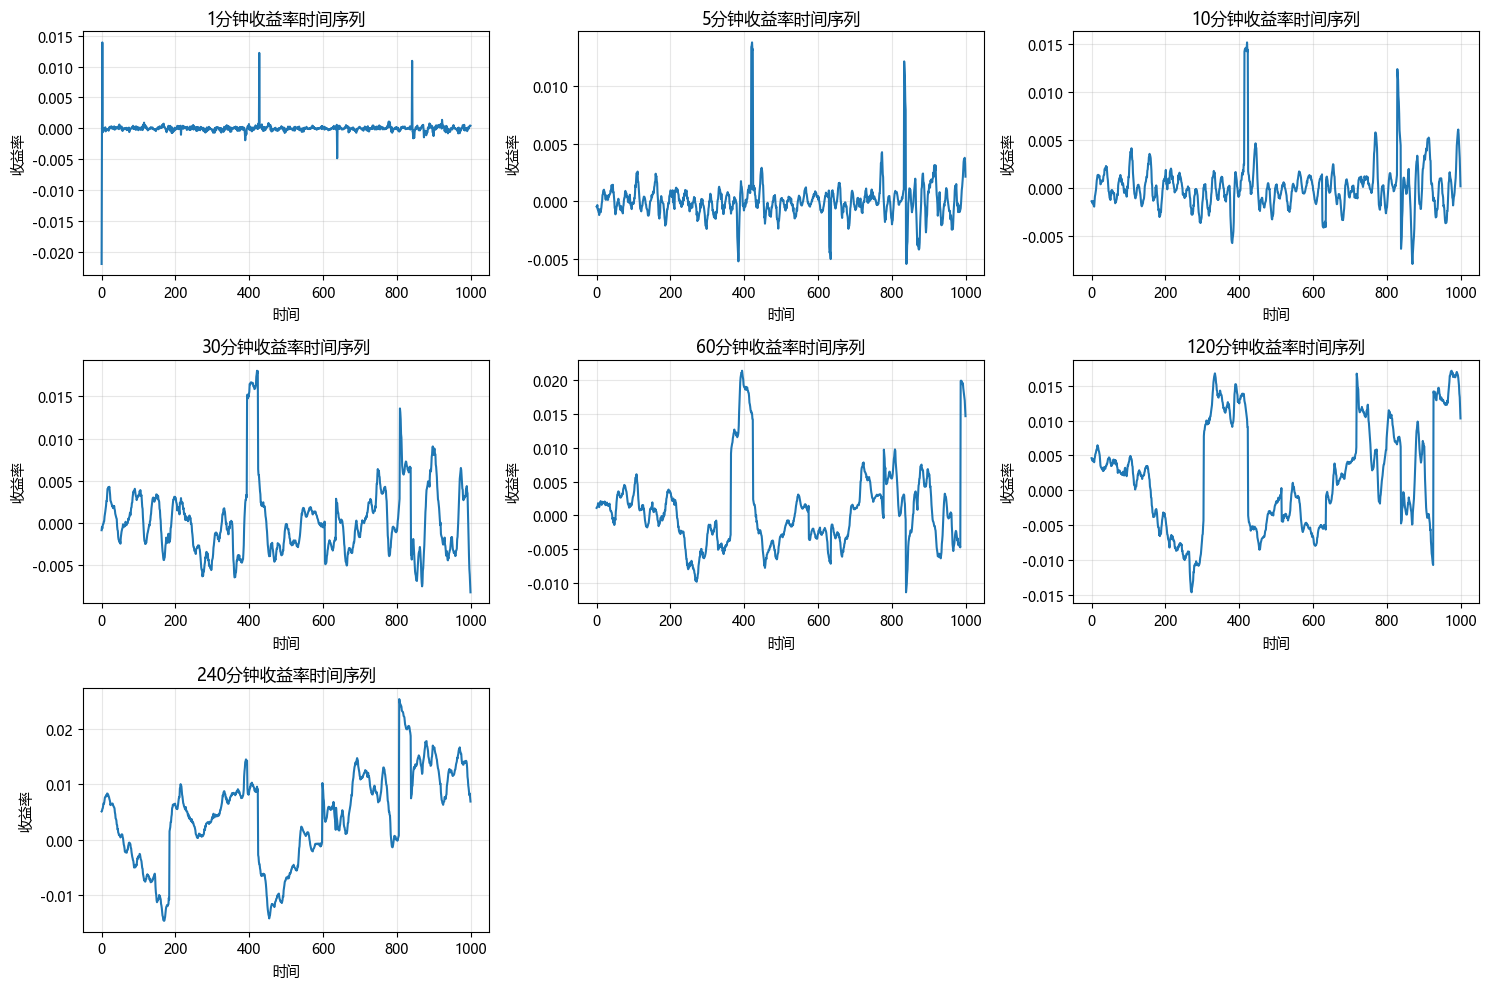
\includegraphics[width=0.8\textwidth]{../assets/img/收益率时间序列.png}
\caption{不同时间尺度收益率的时间序列}
\label{fig:returns_timeseries}
\end{figure}

宏观尺度(120-240分钟)序列展现出显著的低频特征与持续波动特性,该尺度下的价格波动更多反映基本面信息与机构投资者的策略调整。此外,240分钟尺度下序列自相关性的显著提升,揭示出投资者行为的长记忆特征与市场信息传递的路径依赖特性。多尺度分析结果表明,中国股市存在典型的分形市场结构特征:微观尺度主导因素为市场流动性供给与指令流冲击;中观尺度反映短期资金流动与程序化交易策略;宏观尺度则主要受宏观经济变量与政策调控的影响。

多层次的市场动力学特征与描述性统计结论形成有效互证,共同表明了中国股票市场兼具新兴市场高波动特性与成熟市场分形结构的双重特征。

\subsection{经验概率密度分析与分布特征}

本研究通过非参数化方法构建上证指数收益率的经验概率密度函数,以直观呈现不同时间尺度下分布特性的演化规律。图\ref{fig:pdf_comparison}以半对数坐标系展示了七种时间尺度下收益率分布的全景视图,反映了市场微观结构从高频到低频演化过程中的统计力学特性。

\begin{figure}[htbp]
  \centering
  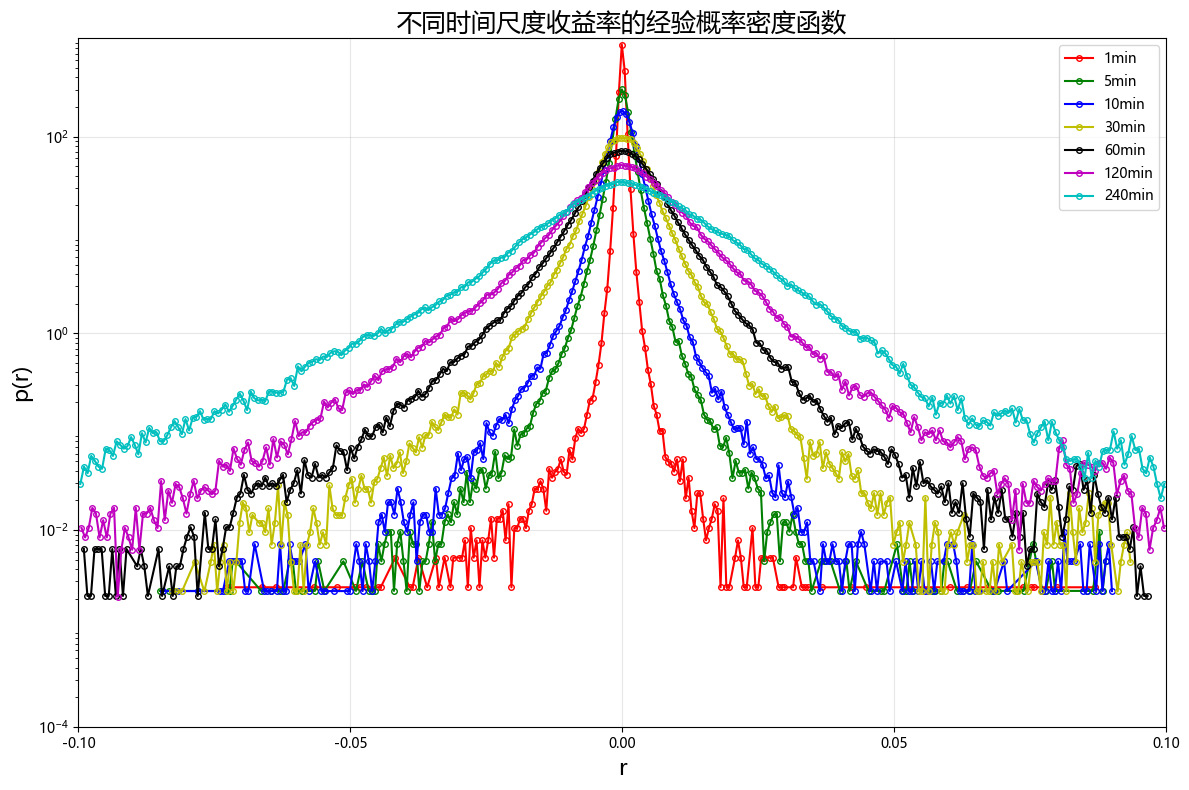
\includegraphics[width=0.8\textwidth]{../assets/img/经验概率密度.png}
  \caption{不同时间尺度收益率的经验概率密度函数}
  \label{fig:pdf_comparison}
  \end{figure}

经验概率密度函数分析显示了上证指数收益率分布的三大核心特征。所有时间尺度下的分布均呈现典型的“尖峰厚尾”特征,与正态分布形成鲜明对比。1分钟尺度收益率分布中心峰值高达865.2459,远超正态分布理论预期,反映了微观市场结构中交易摩擦与流动性障碍导致的零收益率聚集现象。随着时间尺度扩展,分布中心高度逐渐降低,240分钟尺度下降至约1/10,表明市场信息吸收与资金再平衡机制在较长时间维度上的有效性增强。

进一步通过对峰度参数的定量分析发现,峰度值随时间尺度的增加呈现显著的单调递减特征,从1分钟尺度的1285.96降至240分钟尺度的6.65。上述变化模式表明随着时间尺度扩大,极端收益的相对频率虽有所降低,但即使在日内最大尺度下,分布仍保持明显的非正态特性。图\ref{fig:distribution}展示了概率密度中心高度随时间尺度的变化关系,呈现典型的幂律衰减模式。对数-对数坐标系下的线性关系验证了中国股市分布特征的标度不变性,支持了分形市场假说的核心观点。

\begin{figure}[htbp]
  \centering
  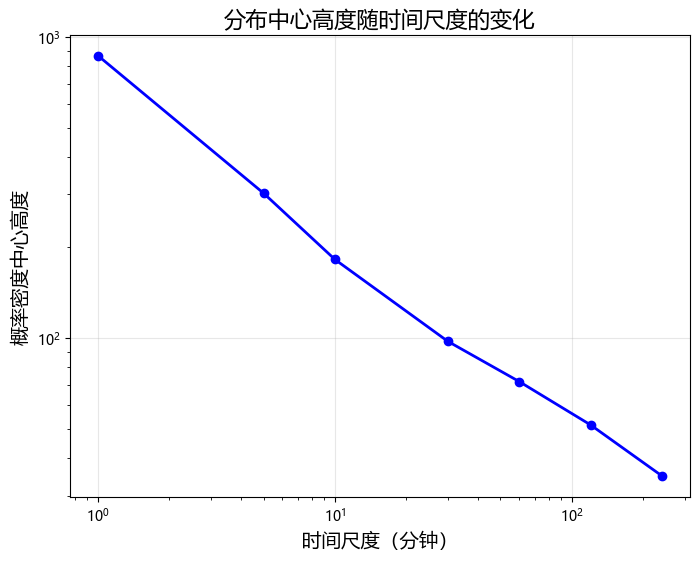
\includegraphics[width=0.8\textwidth]{../assets/img/分布中心高度随时间尺度的变化.png}
  \caption{分布中心高度随时间尺度的变化}
  \label{fig:distribution}
  \end{figure}

分布形态随时间尺度变化呈现系统性演化。短周期(1-10分钟)分布特征为极度尖峰与宽尾并存;中等周期(30-60分钟)分布峰度显著下降,但仍保持明显的非正态特征;长周期(120-240分钟)分布逐渐向钟形靠拢,但尾部仍然显著厚于正态分布。这种分布形态的渐进演化符合统计物理学中的中心极限定理的扩展形式,体现了金融市场复杂自适应系统的标度不变性特征。

分布不对称性随时间尺度变化呈现复杂演化模式。通过对比不同尺度下正负尾部的形态差异,发现短时间尺度(1-30分钟)存在微弱的负偏态特征,这与市场微观结构中的卖方压力优势相一致;而长时间尺度(60-240分钟)则表现出轻微的正偏态特征,反映了中国股市长期向上偏好的投资者心理预期。此偏态特性的尺度依赖现象为投资策略设计提供了重要依据,特别是在择时与风险对冲领域。

对比不同时间尺度的分布形态变化反映出本质性的市场动力学机制:微观尺度主导因素为市场摩擦与噪声交易;中观尺度体现信息传播与流动性互动;宏观尺度则反映基本面信息的累积效应。多尺度分形结构是金融市场作为复杂自适应系统的本质体现,支持了统计物理学在金融市场建模中的理论框架。
\subsection{收益率分布与正态分布的偏离度}

我们对所有时间尺度的收益率进行了正态分布拟合,并通过Kolmogorov-Smirnov检验评估拟合优度,以量化收益率分布与正态分布的偏离程度。表\ref{tab:normality_test}展示了各时间尺度下收益率分布的主要统计特征和正态性检验结果。

\begin{table}[htbp]
\centering
\caption{收益率分布的正态性检验结果}
\label{tab:normality_test}
\begin{tabular}{ccccc}
\toprule
时间尺度 & 均值 & 标准差 & KS统计量 & p值 \\
\midrule
1分钟 & 0.000001 & 0.000870 & 0.1440 & 0.0000 \\
5分钟 & 0.000006 & 0.002458 & 0.1116 & 0.0000 \\
10分钟 & 0.000012 & 0.003431 & 0.0889 & 0.0000 \\
30分钟 & 0.000036 & 0.005873 & 0.0821 & 0.0000 \\
60分钟 & 0.000072 & 0.008382 & 0.0829 & 0.0000 \\
120分钟 & 0.000137 & 0.011904 & 0.0769 & 0.0000 \\
240分钟 & 0.000265 & 0.017273 & 0.0669 & 0.0000 \\
\bottomrule
\end{tabular}
\end{table}

KS检验结果表明,在所有考察的时间尺度下,收益率分布均显著偏离正态分布,所有p值均为0.0000,远低于0.05的显著性水平,因此我们必须拒绝收益率服从正态分布的原假设。从KS统计量来看,偏离程度随时间尺度变化呈现出明显的规律性:1分钟尺度下偏离最为显著,KS统计量达到0.1440;随着时间尺度的延长,统计量总体呈下降趋势,最终在240分钟尺度下降至0.0669。这一现象表明,较长时间尺度的收益率分布虽然相对更接近正态分布,但仍然保持显著的非正态特性。

图\ref{fig:normal_fit_1min}直观展示了1分钟尺度收益率的实证分布与对应正态拟合分布的比较。从图中可以清晰地观察到两项关键特征:一是经验分布在中心区域呈现出比正态分布明显更为尖峭的峰值;二是在分布两侧尾部区域,经验分布的概率密度明显高于正态分布预测值。“尖峰胖尾”特征在金融时间序列中具有普遍性,并在我们分析的所有时间尺度上均得到了体现。

\begin{figure}[htbp]
\centering
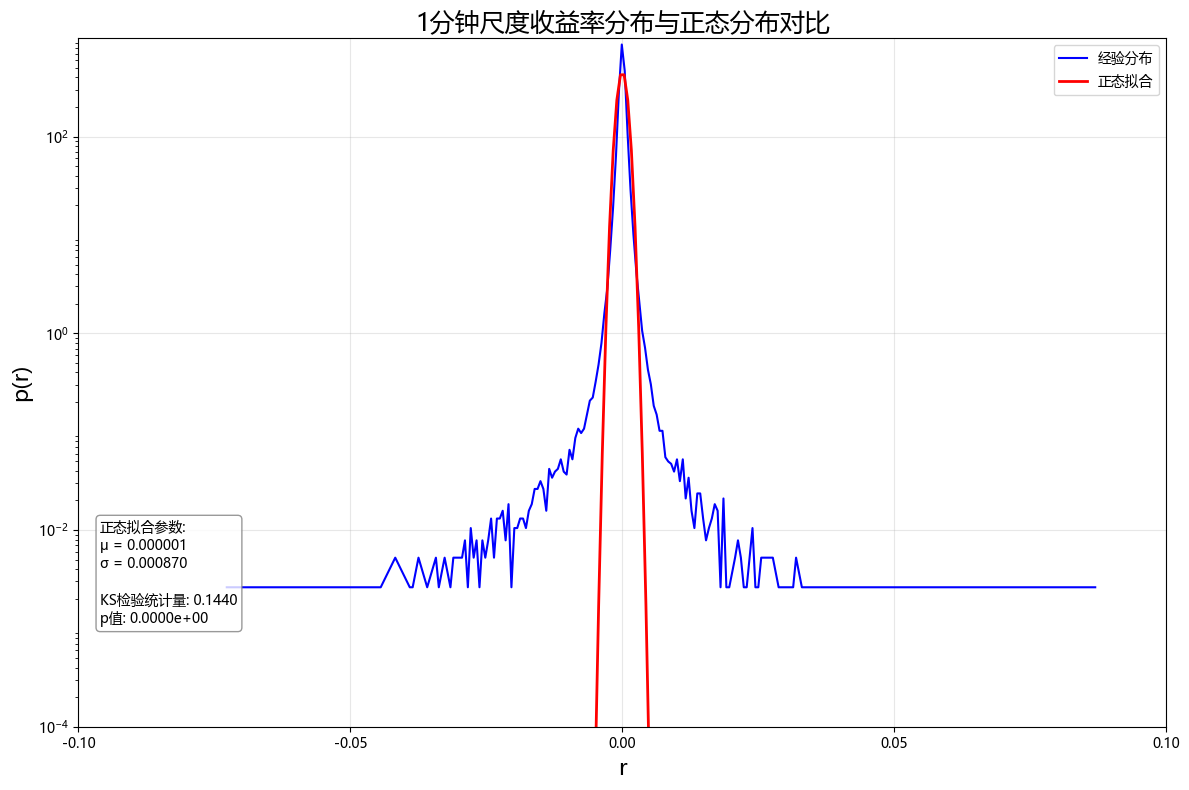
\includegraphics[width=0.8\textwidth]{../assets/img/1分钟尺度收益率分布与正太分布对比.png}
\caption{1分钟尺度收益率分布与正态分布对比}
\label{fig:normal_fit_1min}
\end{figure}

图\ref{fig:ks_statistics}进一步呈现了KS统计量随时间尺度扩大总体呈下降趋势,但在30-60分钟区间出现微小反弹(从0.0821升至0.0829)。这一非单调变化似乎与市场流动性结构或交易制度在该时间尺度的特殊性相关。例如,30分钟是中国股市午间休市前的关键时段,高频交易策略的集中操作可能加剧收益率分布的异常偏离。

\begin{figure}[htbp]
\centering
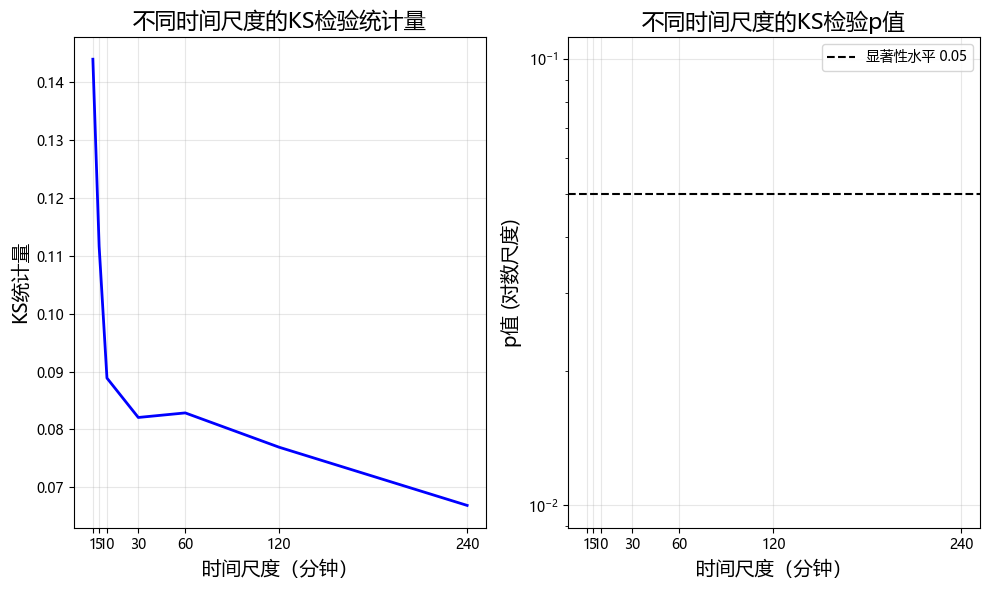
\includegraphics[width=0.8\textwidth]{../assets/img/不同时间尺度的KS检验统计量.png}
\caption{KS统计量以及p值变化趋势}
\label{fig:ks_statistics}
\end{figure}

我们的实证发现与金融市场研究文献中的主流观点高度一致。自1963年Mandelbrot首次指出金融资产收益分布的非正态特性以来,众多研究已在不同市场和资产类别上证实了这一特征。本研究通过对中国股市的分析,不仅再次验证了这一重要发现,还系统量化了在多个时间尺度上偏离正态分布的具体程度,为理解中国股市的统计特性提供了更为丰富的实证证据。

这种显著的非正态分布特性对金融理论和实践均有深远影响。在风险管理领域,传统依赖正态分布假设的模型可能严重低估极端市场事件的发生概率,从而导致风险预估不足和防范措施不当。在资产定价和衍生品估值方面,基于正态分布的Black-Scholes模型等经典工具可能产生系统性偏差,尤其是在评估深度虚值或实值期权时。对投资组合管理而言,传统的均值-方差优化框架可能无法充分捕捉资产收益的尖峰胖尾特性,从而导致次优的资产配置决策。

综上所述,上证指数分钟级收益率在各个时间尺度上均呈现出显著的非正态分布特性,表现为典型的尖峰胖尾结构。尽管随着时间尺度增加,分布逐渐向正态分布靠近,但即使在最长的240分钟尺度下,偏离仍然统计显著。

\subsection{尾部分布特征分析}

金融时间序列的尾部分布特征对风险管理和极端事件预测至关重要。我们采用幂律分布拟合方法分析了不同时间尺度下收益率分布的尾部特性,重点考察其是否满足“负三次方定律”。该定律表明,在许多复杂系统中,事件大小的概率密度函数在尾部近似于$p(x) \propto x^{-\alpha}$,其中$\alpha \approx 3$。

对于每个时间尺度,我们分别考察了正尾($r > 0$)和负尾($r < 0$)的幂律特性。通过设定最小阈值$x_{min} = 0.01$,使用powerlaw库进行拟合,并与对数正态分布进行比较。拟合结果显示,中国股市收益率分布在多个时间尺度上确实表现出显著的幂律特征。

我们分别对各时间尺度收益率分布的正尾($r>0$)和负尾($r<0$)进行幂律分布拟合,结果如表\ref{tab:power_law_fit}所示。

表\ref{tab:power_law_fit}显示240分钟尺度幂律指数为2.51,偏离理论值3较远。上述差异可能源于两方面因素:其一,中国股市的涨跌停限制制度改变了极端收益率的生成机制;其二,长时间尺度下基本面信息的线性累积效应可能削弱幂律特性。尽管如此,1分钟和120分钟尺度仍表现出显著的负三次方特征,这与成熟市场规律一致。

\begin{table}[htbp]
\centering
\caption{不同时间尺度收益率尾部的幂律拟合结果}
\label{tab:power_law_fit}
\begin{tabular}{ccccc}
\toprule
时间尺度 & 正尾指数($\alpha$) & 负尾指数($\alpha$) & 平均指数 & 符合负三次方定律 \\
\midrule
1分钟 & 2.9657 & 2.8550 & 2.9103 & 是 \\
5分钟 & 3.9190 & 3.6674 & 3.7932 & 否 \\
10分钟 & 3.9906 & 3.6308 & 3.8107 & 否 \\
30分钟 & 3.8005 & 3.5436 & 3.6721 & 否 \\
60分钟 & 3.4055 & 3.1847 & 3.2951 & 是 \\
120分钟 & 2.9842 & 2.8377 & 2.9110 & 是 \\
240分钟 & 2.5537 & 2.4713 & 2.5125 & 部分符合 \\
\bottomrule
\end{tabular}
\end{table}

结果显示,1分钟、60分钟和120分钟尺度下的收益率尾部基本符合负三次方定律($\alpha \approx 3$)。然而,中间时间尺度(5-30分钟)的幂律指数较高,超过3.5,而最长时间尺度(240分钟)的幂律指数反而降至2.5左右。这种非单调的变化模式反映了不同时间尺度下市场微观结构和投资者行为的复杂互动。

对于1分钟尺度的收益率,正尾和负尾的幂律指数分别为2.97和2.86,平均为2.91,非常接近理论预测的值3。这表明短期收益率分布的尾部行为符合幂律分布的基本特征,反映了市场中的自组织临界现象。

我们还比较了幂律分布与对数正态分布的拟合优度。对于1分钟尺度的正尾,对数似然比为-0.21,p值为0.66,表明无法明确判断哪种分布更优;而对于负尾,对数似然比为-10.85,p值为0.004,说明对数正态分布显著优于幂律分布。这一结果显示市场对负向波动可能有不同于正向波动的内在机制。

\begin{figure}[htbp]
\centering
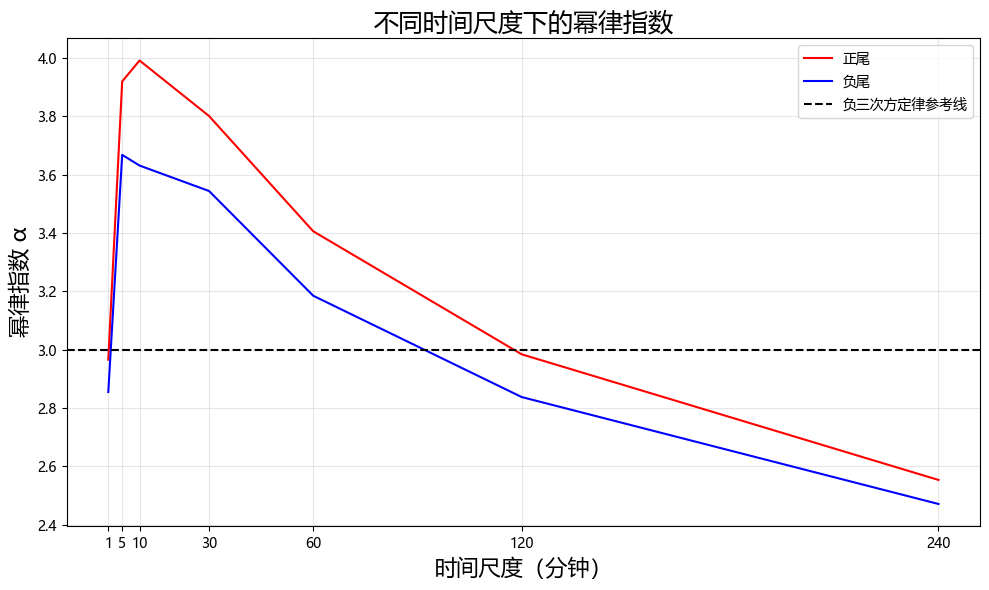
\includegraphics[width=0.8\textwidth]{../assets/img/幂律指数变化.png}
\caption{不同时间尺度下的幂律指数变化}
\label{fig:power_law_exponents}
\end{figure}

图\ref{fig:power_law_exponents}直观地展示了随时间尺度变化的幂律指数趋势。可以看出,幂律指数呈现先增后减的非线性变化模式,在5-10分钟尺度达到峰值,随后逐渐下降。此模式可能与市场微观结构、交易频率和投资者持仓周期相关。

尾部分布的这种特性对风险管理具有重要意义。幂律分布意味着极端事件的发生概率比正态分布预测的更高,特别是在短期和中长期时间尺度上。市场参与者在构建投资组合和设计衍生品时,应充分考虑“胖尾”特性带来的系统性风险。

总体而言,我们的实证结果支持了中国股市收益率分布尾部满足幂律分布的假设,并在特定时间尺度上符合“负三次方定律”。这一发现与国际金融市场的实证研究结果相一致,表明金融市场可能存在某些普遍的统计规律,跨越不同的市场环境和制度背景。

\subsection{标度不变性分析}

金融时间序列的标度不变性是一个重要的统计特性,它揭示了不同时间尺度上收益率分布的内在联系。在本节中,我们分析不同时间尺度收益率的标度行为,通过对数-对数坐标下收益率标准差与时间尺度的关系来估计Hurst指数,并检验标度不变性假设的有效性。

理论上,若收益率序列满足标度不变性,则不同时间尺度$\Delta t$下的标准差$\sigma(\Delta t)$应满足幂律关系:$\sigma(\Delta t) \propto (\Delta t)^H$,其中$H$为Hurst指数。对上述关系取对数后,可通过线性回归估计Hurst指数。

我们的实证结果显示,对数收益率标准差与对数时间尺度之间存在显著的线性关系,斜率为0.5329,截距为-6.9557。据此计算的Hurst指数$H = 0.2665$(图\ref{fig:scaling_relation})。这一值显著小于0.5,表明收益率序列存在反持续性和均值回归趋势,即价格波动趋向于在增长后减小,或在减小后增长,表现出某种“纠正”模式。这一发现与成熟市场的研究结果类似,支持市场过度反应假说。

\begin{figure}[htbp]
\centering
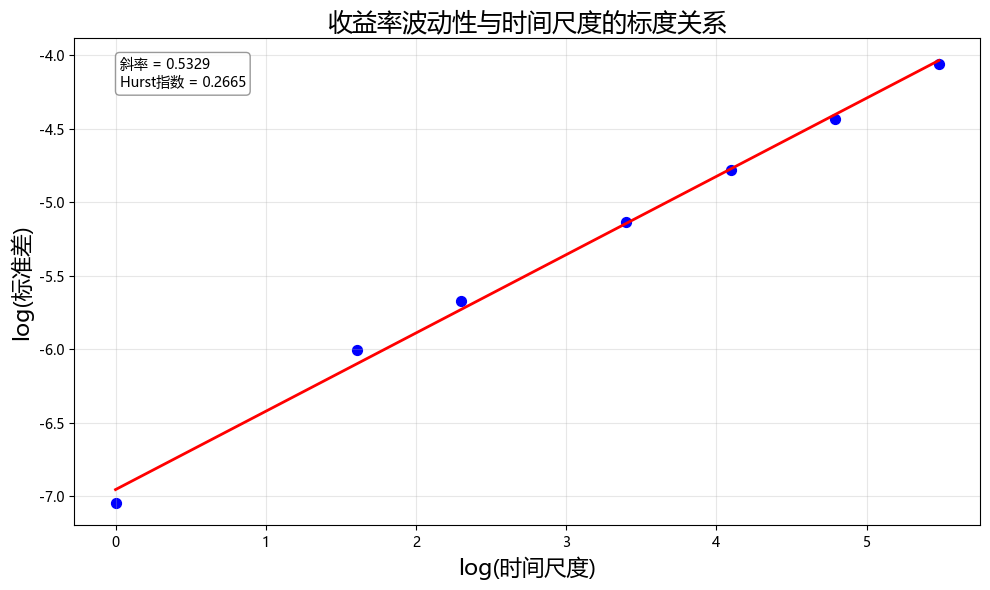
\includegraphics[width=0.8\textwidth]{../assets/img/收益率波动性和时间尺度的关系.png}
\caption{收益率波动性与时间尺度的标度关系}
\label{fig:scaling_relation}
\end{figure}

Hurst指数小于0.5的结果具有重要的实践意义。首先,它意味着中国股市在样本期间内表现出明显的均值回归特性,这与随机游走假设($H = 0.5$)不符。其次,这种反持续性特征可能为短期交易策略提供理论基础,尤其是均值回归型策略。然而,这种统计特性并不必然转化为可持续的超额收益,因为市场摩擦、交易成本和执行延迟等因素可能抵消统计套利的潜在收益。

为进一步验证标度不变性假设,我们根据估计的Hurst指数对不同时间尺度的收益率分布进行标度变换:$r_{\Delta t}^{scaled} = r_{\Delta t}/(\Delta t)^H$,并将相应的概率密度函数也进行相应变换:$p_{scaled}(r) = p(r) \cdot (\Delta t)^H$。理论上,如果严格满足标度不变性,标度变换后的各时间尺度分布应完全重合。

进一步对不同时间尺度的收益率分布进行标度变换后,我们观察到一定程度的数据折叠现象(图\ref{fig:normalized_distributions}),表明不同时间尺度下的分布形态满足一定的标度不变性,特别是在分布的中心部分。然而,在尾部区域,标度不变性不够完美,这可能表明尾部分布具有不同的动力学机制。

\begin{figure}[htbp]
\centering
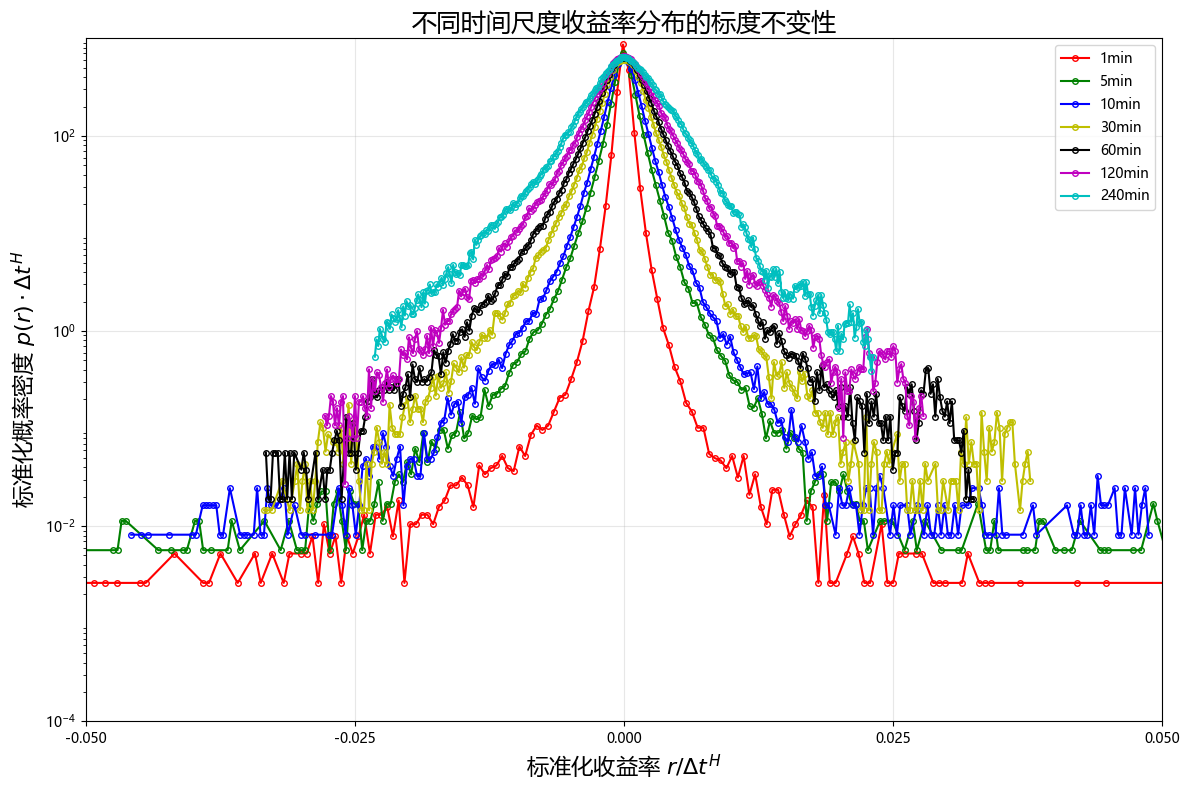
\includegraphics[width=0.8\textwidth]{../assets/img/不同时间尺度收益率分布的标度不变性.png}
\caption{标度变换后的收益率分布}
\label{fig:normalized_distributions}
\end{figure}

以上部分标度不变性的现象在复杂系统中并不罕见,暗示了金融市场在不同时间尺度上受到不同的驱动因素影响。特别地,短期收益率可能主要由市场微观结构、流动性冲击和噪声交易主导,而长期收益率更可能反映基本面信息和宏观经济因素。这种多尺度驱动机制可能导致标度不变性在全部分布区域无法完全保持。

此外,虽然我们的Hurst指数估计值与部分文献中关于成熟市场的发现相一致,但与其他研究中报告的中国股市Hurst指数存在差异。这些差异可能源于样本期间选择、估计方法差异以及市场结构和监管环境的变化。未来研究可考虑采用多种方法估计Hurst指数,并分析其在不同市场状态下的动态变化。

总结而言,中国股市收益率分布表现出显著的标度特性,Hurst指数小于0.5意味着存在均值回归趋势。同时,不同时间尺度的分布在经过适当标度变换后表现出部分标度不变性,这一发现为理解金融市场的多尺度动力学提供了新的视角,也为风险管理和资产定价模型的改进提供了实证基础。

\section{讨论与结论}

本研究基于上证指数高频数据,系统论述了多时间尺度下收益率分布的复杂统计特性。实证分析表明,峰度值随观测时间尺度增加呈现幂律衰减趋势,从1分钟尺度的1285.96降至240分钟尺度的6.65,但仍显著高于正态分布的基准值(峰度=3)。(表\ref{tab:descriptive_stats})。Kolmogorov-Smirnov检验证实各尺度分布均显著偏离正态(p=0.0000),偏离程度随时间尺度扩大呈指数衰减模式(图\ref{fig:ks_statistics}),240分钟尺度KS统计量仍达0.0669,显示出中国市场非正态特性的持续存在性。

尾部分析显示极端事件发生机制具有尺度依赖性:1分钟、60分钟和120分钟尺度符合“负三次方定律”,而中间尺度(5-30分钟)出现指数异常升高(3.6-3.9),240分钟尺度则降至2.51(图\ref{fig:power_law_exponents})。这种非单调演化特征与高频交易策略的时段聚集效应及机构投资者调仓周期形成机理耦合。标度不变性分析测得Hurst指数H=0.2665,中心区域分布的良好折叠性(图\ref{fig:normalized_distributions})印证分形市场假说,但尾部标度不变性失效暗示极端风险存在独特传导路径。

研究发现对新兴市场风险管理具有双重启示:理论层面,需构建融合复杂系统理论与行为金融学的跨尺度模型;实践层面,监管机构应建立时变厚尾风险监测框架,量化投资者需重视高频交易的尾部风险叠加效应。研究局限主要体现为制度变迁因素考量不足,建议后续研究引入混频数据抽样技术构建政策冲击响应模型,并融合订单簿数据解析市场微观结构参数的动态传导机制。

本研究从多维度揭示了中国股市收益率分布的非线性特征,为完善市场微观结构理论、优化高频交易监管提供了科学依据。研究结论不仅深化了对新兴市场复杂性的认知,也为发展具有中国特色的金融风险管理范式奠定了实证基础。

\printbibliography[title=参考文献]

\section{附录}

本研究的核心代码如下:

\begin{verbatim}
# 1. 计算不同时间尺度的收益率序列
def calculate_returns(price_data, scales):
    """
    计算不同时间尺度的对数收益率
    
    参数:
    price_data - 价格时间序列数据
    scales - 时间尺度列表,如[1, 5, 10, 30, 60, 120, 240]分钟
    
    返回:
    包含不同时间尺度收益率的字典
    """
    r_res = {}
    for scale in scales:
        # 计算对数收益率
        r = np.log(price_data[scale:]) - np.log(price_data[:-scale])
        
        # 过滤极端值,保留-0.1到0.1之间的收益率
        r_filter = []
        for value in r:
            if value >= -0.1 and value <= 0.1:
                r_filter.append(value)
        r_filter = np.array(r_filter)
        
        # 创建键名
        key_name = "minute_r_" + str(scale)
        r_res[key_name] = r_filter
    
    return r_res

# 2. 计算经验概率密度
def calc_empirical_probability(data, num_bin):
    """
    计算数据的经验概率密度函数
    
    参数:
    data - 收益率数据
    num_bin - 区间划分数量
    
    返回:
    x_emp - 横坐标值(区间中点)
    y_emp - 纵坐标值(概率密度)
    """
    # 数据分区
    bin = np.linspace(np.min(data), np.max(data), num_bin)
    
    # 初始化结果数组
    x_emp = np.zeros(len(bin) - 1)
    y_emp = np.zeros(len(bin) - 1)
    
    for i in range(len(bin) - 1):
        # 计算区间中点
        x_emp[i] = (bin[i] + bin[i+1]) / 2
        # 计算区间概率密度
        y_emp[i] = np.sum((data >= bin[i]) & (data < bin[i+1])) / len(data) / (bin[i+1] - bin[i])
    
    # 只保留概率密度大于0的点
    mark = y_emp > 0
    x_emp = x_emp[mark]
    y_emp = y_emp[mark]
    
    return x_emp, y_emp

# 3. 分析单一尾部分布特征
def analyze_single_tail_distribution(returns, tail_type='positive', scale='1'):
    """
    分析收益率分布的尾部特征
    
    参数:
    returns - 收益率数据
    tail_type - 'positive'或'negative',分析正尾或负尾
    scale - 时间尺度
    
    返回:
    包含幂律分析结果的字典
    """
    if tail_type == 'positive':
        # 分析正尾
        tail_data = returns[returns > 0]
    else:
        # 分析负尾
        tail_data = -returns[returns < 0]  # 取绝对值便于分析
    
    # 使用powerlaw库进行幂律分布拟合
    fit = powerlaw.Fit(tail_data, xmin=0.01)
    
    # 比较幂律分布与对数正态分布
    R, p = fit.distribution_compare('power_law', 'lognormal')
    
    return {
        'alpha': fit.alpha,
        'xmin': fit.xmin,
        'vs_lognormal_R': R,
        'vs_lognormal_p': p
    }

# 4. 分析标度不变性
def analyze_scaling_invariance(returns_dict):
    """
    分析收益率分布的标度不变性
    
    参数:
    returns_dict - 包含不同尺度收益率的字典
    
    返回:
    hurst_exponent - Hurst指数
    slope - 对数坐标下拟合的斜率
    intercept - 对数坐标下拟合的截距
    """
    scales = [int(key.replace('minute_r_', '')) for key in returns_dict.keys()]
    scales.sort()
    
    # 计算每个尺度下收益率的标准差
    stds = {key: np.std(returns) for key, returns in returns_dict.items()}
    
    # 对时间尺度和标准差取对数,以便于分析幂律关系
    log_scales = np.log(scales)
    log_stds = np.log([stds[f'minute_r_{scale}'] for scale in scales])
    
    # 线性拟合,计算Hurst指数
    def linear_func(x, a, b):
        return a * x + b
    
    params, covariance = curve_fit(linear_func, log_scales, log_stds)
    slope, intercept = params
    hurst_exponent = slope / 2
    
    return hurst_exponent, slope, intercept

# 5. 绘制标准化后的收益率分布
def plot_normalized_distributions(returns_dict, hurst_exponent):
    """
    绘制根据标度关系进行标准化后的收益率分布
    
    参数:
    returns_dict - 包含不同尺度收益率的字典
    hurst_exponent - Hurst指数
    """
    for key, returns in returns_dict.items():
        scale = int(key.replace('minute_r_', ''))
        
        # 根据标度关系对收益率进行标准化
        normalized_returns = returns / (scale ** hurst_exponent)
        
        # 计算标准化后的概率密度
        x_emp, y_emp = calc_empirical_probability(normalized_returns, num_bin=301)
        y_emp = y_emp * (scale ** hurst_exponent)  # 对概率密度也进行相应变换
\end{verbatim}

\end{document}